%! TeX program = lualatex
\documentclass[12pt,a4paper]{article}

\usepackage[nil]{babel}
\usepackage{unicode-math}
\usepackage[svgnames]{xcolor}
\usepackage{lmodern}
\usepackage{graphicx}
\usepackage{wrapfig}
\usepackage{float}
\usepackage{parskip}

\babelprovide[import=el, main, onchar=ids fonts]{greek} % can also do import=el-polyton
\babelprovide[import, onchar=ids fonts]{english}

\babelfont{rm}
          [Language=Default]{Liberation Sans}
\babelfont[english]{rm}
          [Language=Default]{Liberation Sans}
\babelfont{sf}
          [Language=Default]{Liberation Sans}
\babelfont{tt}
          [Language=Default]{Liberation Sans}

%Enter Title Here
 \title{Robustness-diagrams-v0.1 \\ LibShare}
\author{\textbf{Ονόματα / ΑΜ / Έτος:} \\ Γρηγόρης Καπαδούκας / 1072484 / 4\textdegree \\ Χρήστος Μπεστητζάνος / 1072615 / 4\textdegree \\ Νικόλαος Αυγέρης / 1067508 / 5\textdegree \\ Περικλής Κοροντζής / 1072563 / 4\textdegree}

\begin{document}

\makeatletter
\begin{center}
	\LARGE{\@title} \\
	\pagebreak
    \begin{LARGE}\@author\end{LARGE}
    \pagebreak
\end{center}

%Insert Body Here
\section{Robustness Diagrams}

\subsection{Αναζήτηση βιβλίων / χρήστη / αιτήσεων}
\begin{figure}[H]
	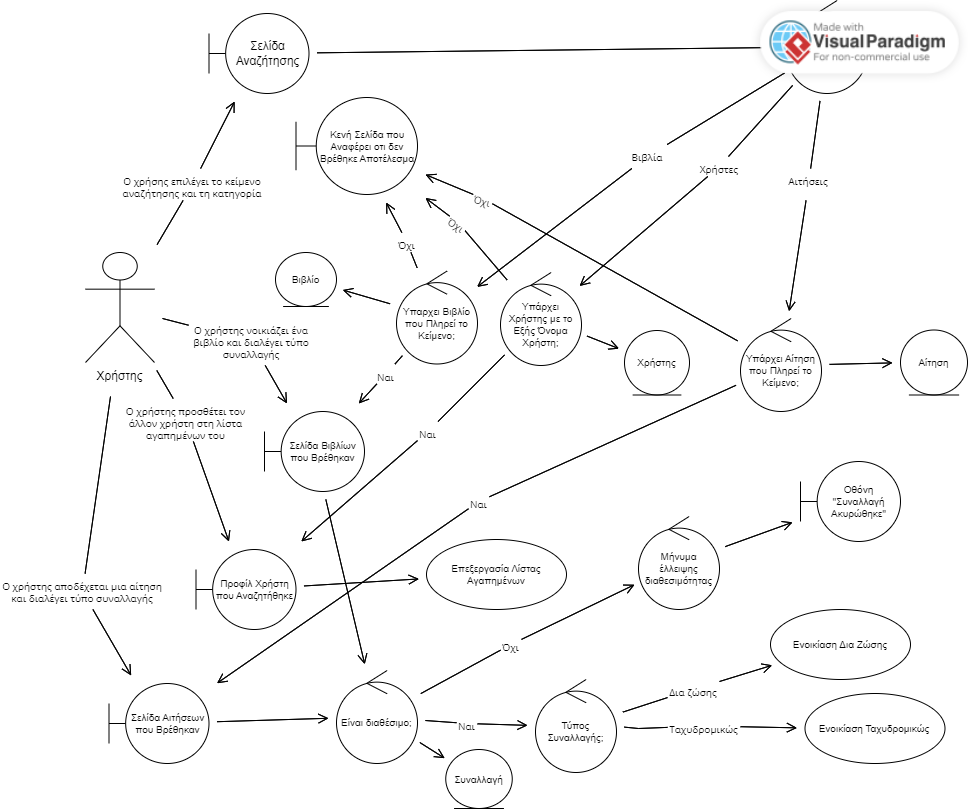
\includegraphics[width=\textwidth]{Search Robustness.png}
	\caption{Robustness Diagram: Αναζήτηση βιβλίων / χρήστη / αιτήσεων}
	\label{Robustness Diagram: Αναζήτηση βιβλίων / χρήστη / αιτήσεων}
\end{figure}

\subsection{Ενοικίαση βιβλίου από άλλο χρήστη}
\begin{figure}[H]
	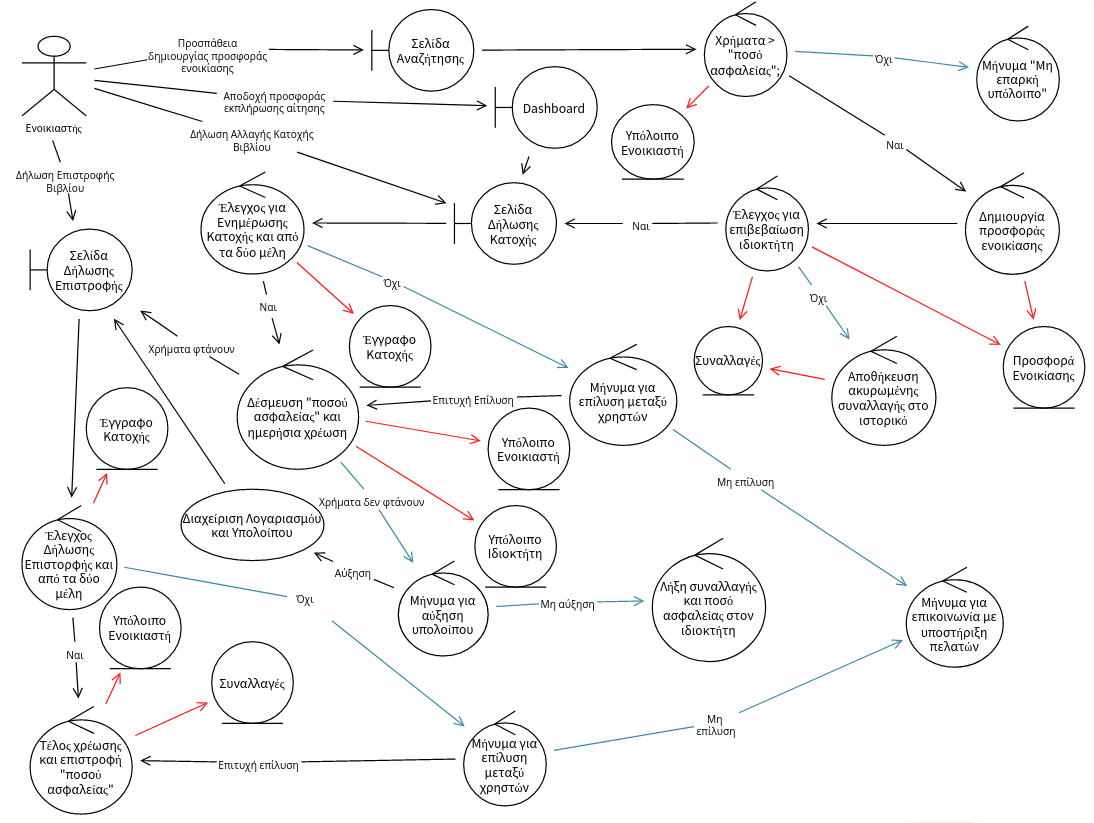
\includegraphics[width=\textwidth]{Rent from User Robustness.png}
	\caption{Robustness Diagram: Ενοικίαση βιβλίου από άλλο χρήστη}
	\label{Robustness Diagram: Ενοικίαση βιβλίου από άλλο χρήστη}
\end{figure}

\subsection{Ενοικίαση βιβλίου σε άλλο χρήστη (μεριά ιδιοκτήτη)}
\begin{figure}[H]
	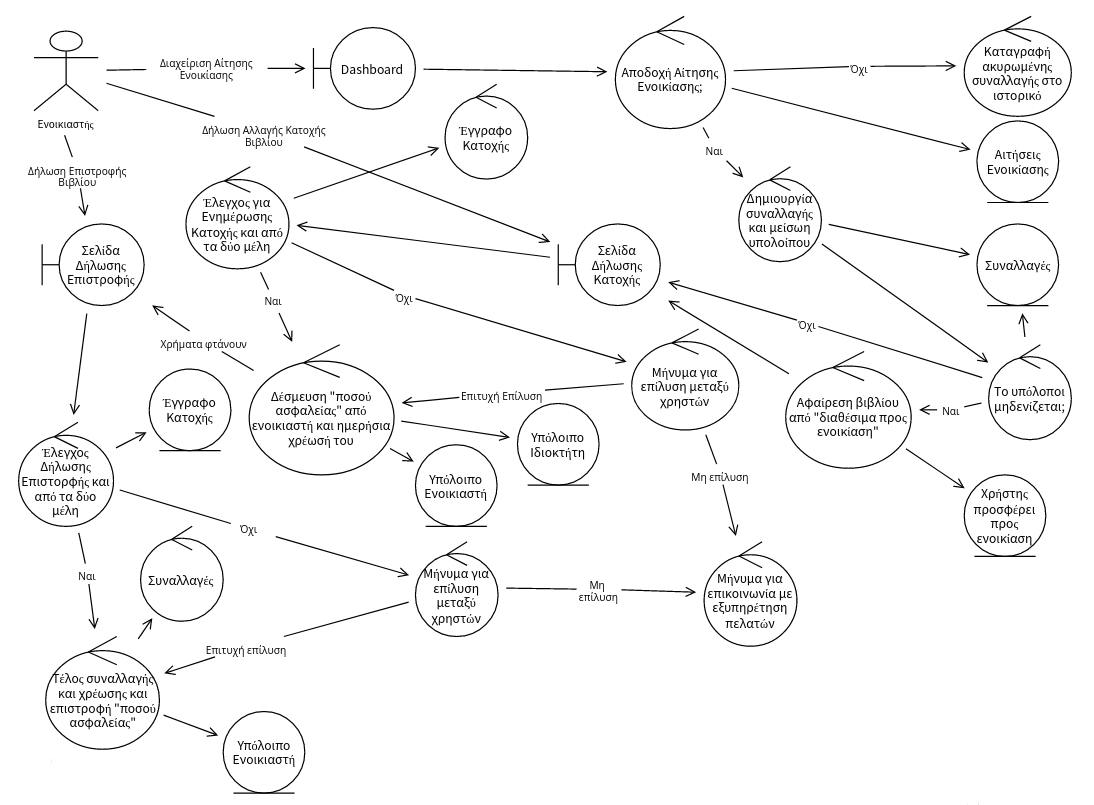
\includegraphics[width=\textwidth]{Rent to User Robustness.png}
	\caption{Robustness Diagram: Ενοικίαση βιβλίου σε άλλο χρήστη (μεριά ιδιοκτήτη)}
	\label{Robustness Diagram: Ενοικίαση βιβλίου σε άλλο χρήστη μεριά ιδιοκτήτη}
\end{figure}

\end{document}
